\appendixpage
\appendix
\chapter*{Appendices}
\addcontentsline{toc}{chapter}{List of Appendices}
\renewcommand{\thesection}{\Alph{section})}
\renewcommand{\thesubsection}{\Alph{section}.\arabic{subsection}}

\section{Verbose Queue Length Stabilisation Results Over LS Update Intervals}
\subsection{Average Queue Length}
    \begin{figure}[h]
        \centering
        \begin{subfigure}[b]{0.475\textwidth}
            \centering
            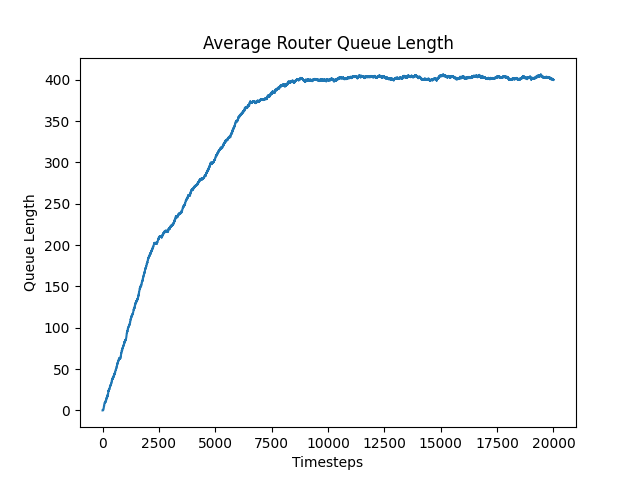
\includegraphics[width=\textwidth]{figs/appendix/average_ls=1.png}
            \caption[]{Average router queue length (LS update interval = 1)}
        \end{subfigure}
        \hfill
        \begin{subfigure}[b]{0.475\textwidth}
            \centering
            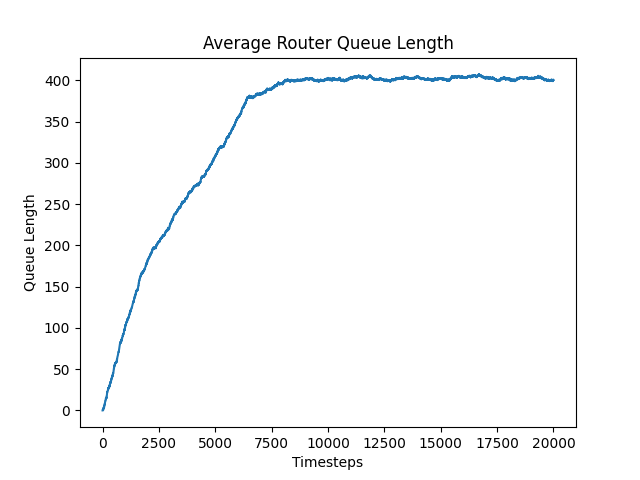
\includegraphics[width=\textwidth]{figs/appendix/average_ls=10.png}
            \caption[]{Average router queue length (LS update interval = 10)}
        \end{subfigure}
    \end{figure}
    \begin{figure}[H]\ContinuedFloat
        \centering
        \begin{subfigure}[b]{0.475\textwidth}
            \centering
            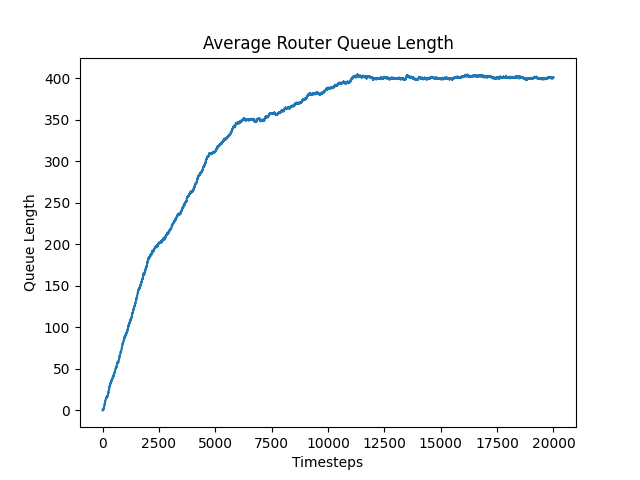
\includegraphics[width=\textwidth]{figs/appendix/average_ls=50.png}
            \caption[]{Average router queue length (LS update interval = 250)}
        \end{subfigure}
        \hfill
        \begin{subfigure}[b]{0.475\textwidth}
            \centering
            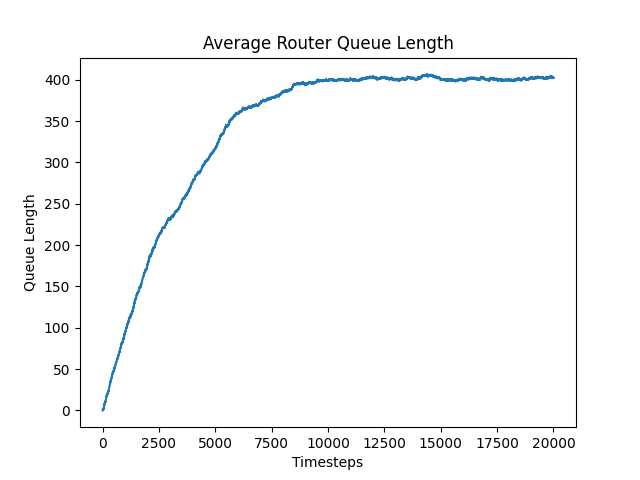
\includegraphics[width=\textwidth]{figs/appendix/average_ls=500.png}
            \caption[]{Average router queue length (LS update interval = 500)}
        \end{subfigure}
    \end{figure}
    \begin{figure}[H]\ContinuedFloat
        \centering
        \begin{subfigure}[t]{0.475\textwidth}
            \centering
            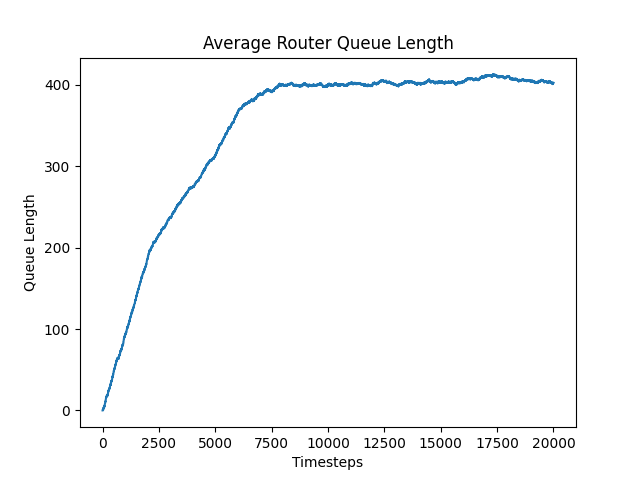
\includegraphics[width=\textwidth]{figs/appendix/average_ls=1000.png}
            \caption[]{Average router queue length (LS update interval = 1000)}
            \label{fig:avgq-1000}
        \end{subfigure}
        \hfill
        \begin{subfigure}[t]{0.475\textwidth}
            \centering
            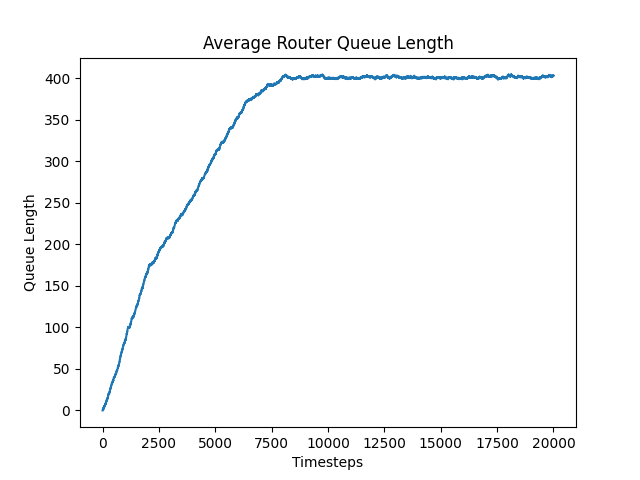
\includegraphics[width=\textwidth]{figs/appendix/average_ls=10000.png}
            \caption[]{Average router queue length (LS update interval = 10000)}
            \label{fig:avgq-10000}
        \end{subfigure}
    \end{figure}
    
\subsection{Variance of Queue Length}
\lfix{Trim variance graphs to same length as averages}
    \begin{figure}[H]
        \centering
        \begin{subfigure}[b]{0.475\textwidth}
            \centering
            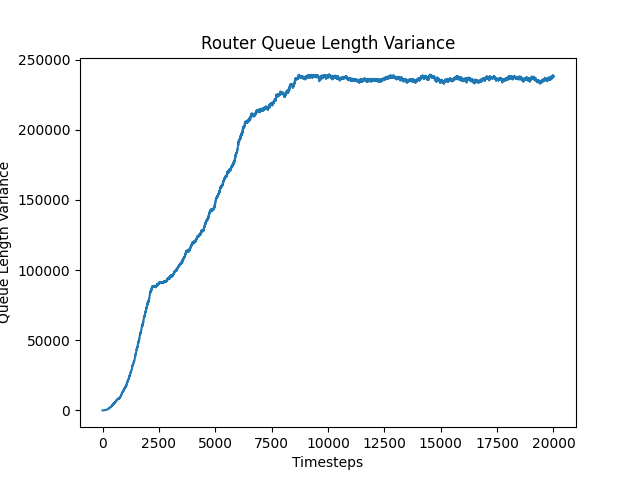
\includegraphics[width=\textwidth]{figs/appendix/variance_ls=1.png}
            \caption[]{Variance of router queue length (LS update interval = 1)}
            \label{fig:qvar-1}
        \end{subfigure}
        \hfill
        \begin{subfigure}[b]{0.475\textwidth}
            \centering
            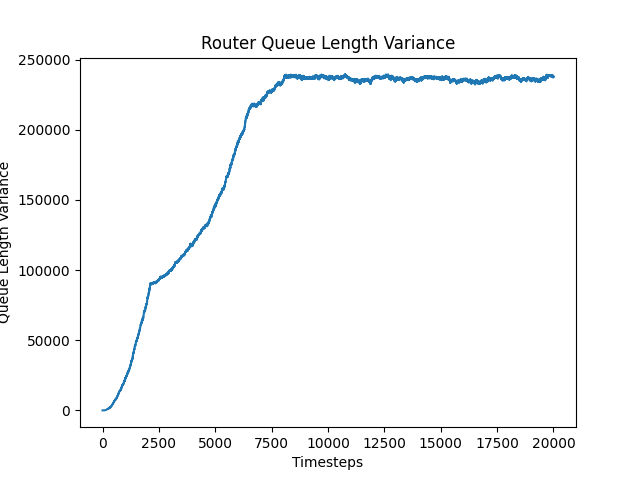
\includegraphics[width=\textwidth]{figs/appendix/variance_ls=10.png}
            \caption[]{Variance of router queue length (LS update interval = 10)}
            \label{fig:qvar-10}
        \end{subfigure}
    \end{figure}
    \begin{figure}[H]\ContinuedFloat
        \centering
        \begin{subfigure}[b]{0.475\textwidth}
            \centering
            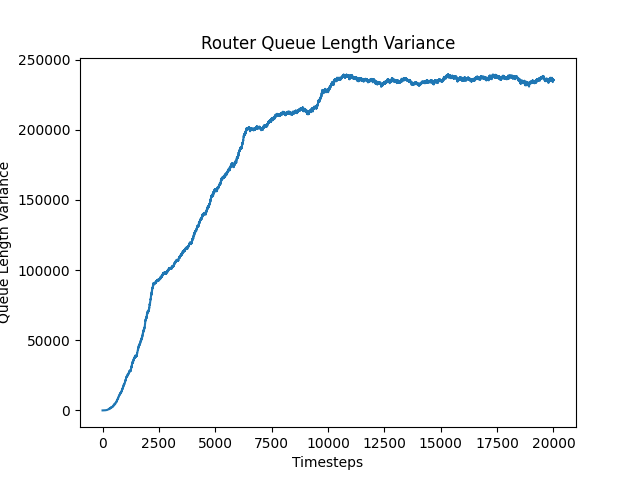
\includegraphics[width=\textwidth]{figs/appendix/variance_ls=250.png}
            \caption[]{Variance of router queue length (LS update interval = 250)}
            \label{fig:qvar-250}
        \end{subfigure}
        \hfill
        \begin{subfigure}[b]{0.475\textwidth}
            \centering
            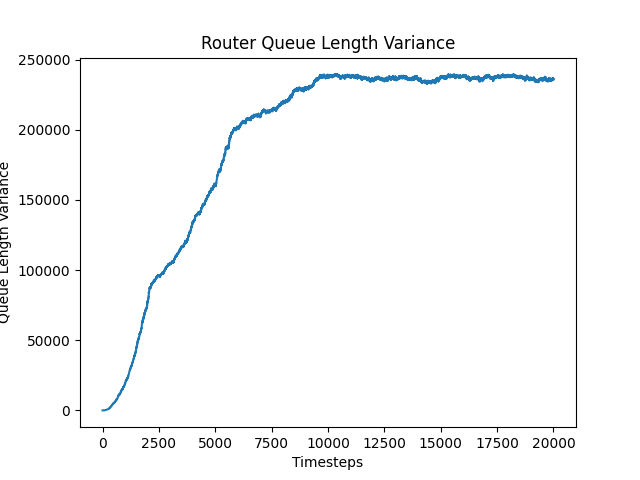
\includegraphics[width=\textwidth]{figs/appendix/variance_ls=500.png}
            \caption[]{Variance of router queue length (LS update interval = 500)}
            \label{fig:qvar-500}
        \end{subfigure}
    \end{figure}
    \begin{figure}[H]\ContinuedFloat
        \begin{subfigure}{0.475\textwidth}
            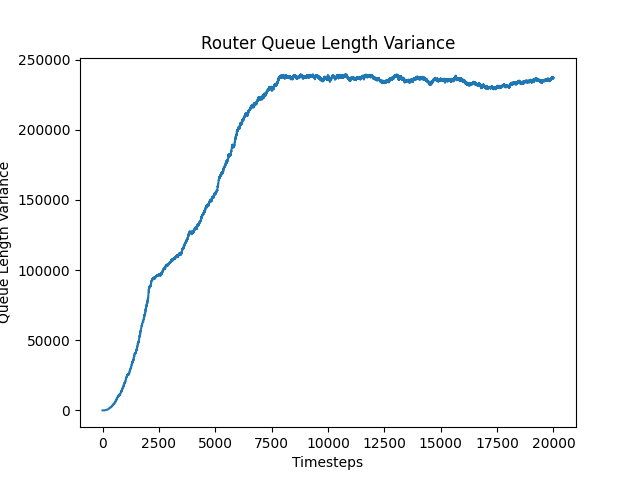
\includegraphics[width=\textwidth]{figs/appendix/variance_ls=1000.png}
            \caption[]{Variance of router queue length (LS update interval = 1000)}
            \label{fig:qvar-1000}
        \end{subfigure}
        \hfill
        \begin{subfigure}[H]{0.475\textwidth}
            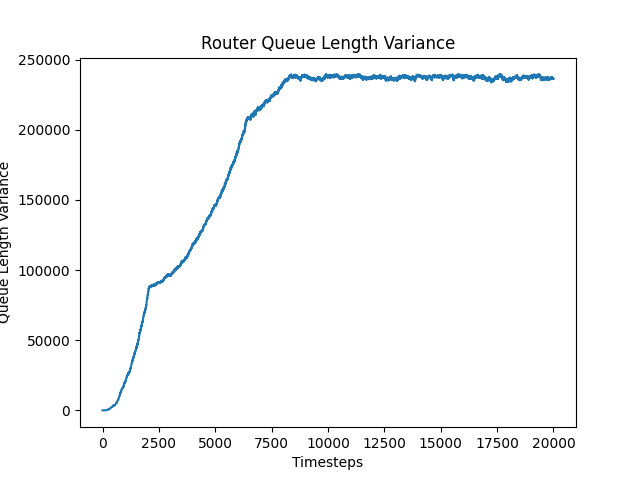
\includegraphics[width=\textwidth]{figs/appendix/variance_ls=10000.png}
            \caption[]{Variance of router queue length (LS update interval = 10000)}
            \label{fig:qvar-10000}
        \end{subfigure}
    \end{figure}

\newpage

\newpage
\section{Queue Stabilization}
\label{sec:Aqueuestabilization}

\todo{Describe how we generated results for steady queue lengths, implementation of link state routing and update interval in the model}

\captionsetup{justification=centering}
\begin{figure}[H]
    \centering
    \begin{subfigure}{0.475\textwidth}
        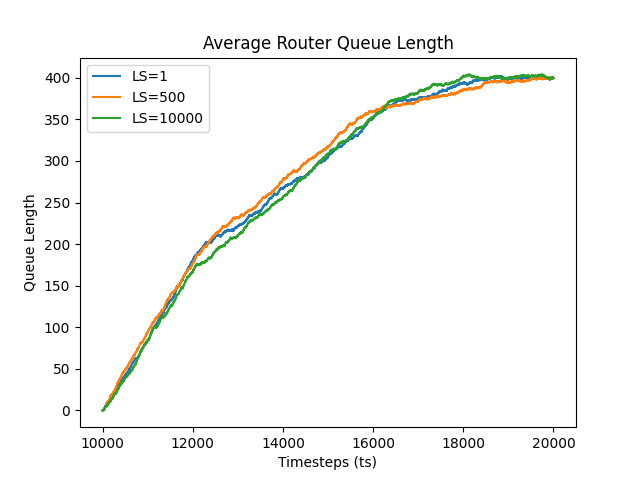
\includegraphics[width=\textwidth]{figs/appendix/average_of_1,500,10000.png}
        \caption{Average.}
        \label{fig:Ravgq}
    \end{subfigure}
    \hfill
    \begin{subfigure}{0.475\textwidth}
        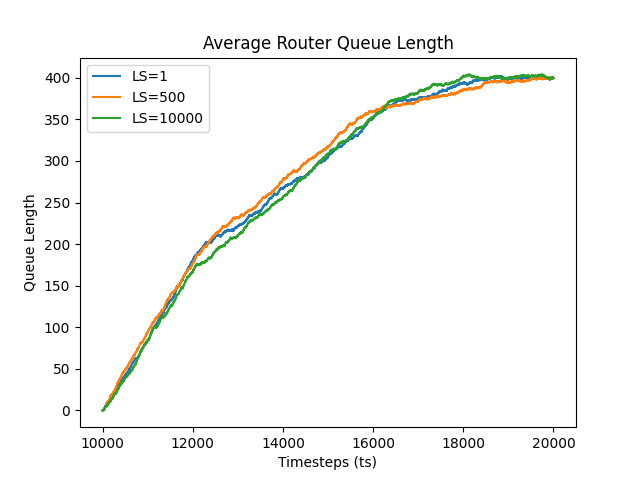
\includegraphics[width=\textwidth]{figs/appendix/average_of_1,500,10000.png}
        \caption[]{Variance.}
        \label{fig:Rvarq}
    \end{subfigure}
    \caption{Mean and variance of router queue buffer lengths over link-state update intervals 1, 500, and 10,000].}
\end{figure}

\begin{table}[H]
    \centering\sisetup{table-number-alignment=center}
    \begin{tabular}{@{}lS[table-format=1.2e1]c@{}}
        \toprule
        \multirow{2}{*}{\makecell{LS Update \\ Interval}} & \multicolumn{2}{@{}S@{}}{\textbf{Time-step range}}\\
        \cmidrule(rl){2-3}
        & {$\leq$ 20,000} & {> 20,000} \\
        \midrule
        1       & 1.07E4 & 6.25 \\ 
        10      & 1.02e4 & 4.88 \\
        50      & 1.01e4 & 3.21 \\
        250     & 1.07e4 & 5.06 \\
        500     & 1.01e4 & 6.05 \\
        1,000   & 1.03e4 & 3.47 \\
        10,000  & 1.12e4 & 5.22 \\
        \bottomrule
    \end{tabular}
    \caption{Variance pre and post queue length stabilization point}
\end{table}

\newpage

\newpage
\section{Sympathetic Packet Delay Metric Increase}
\label{sec:Asympathicpdv}
Note symmetric increase due to topology symmetry.

\newpage
\section{Curve Fitting with Alternative Minimisation Algorithms}
\label{Aaltcurvefit}
\begin{figure}[H]
    \centering
    \begin{subfigure}{0.475\textwidth}
        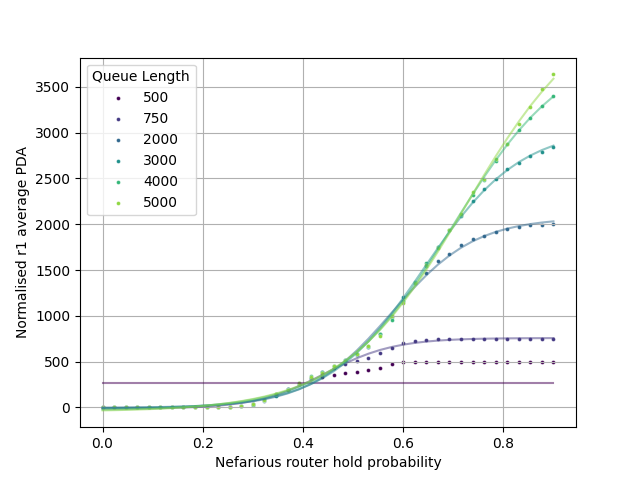
\includegraphics[width=\textwidth]{figs/results/qlen_fitting/qlen_PDA_trf.png}
        \caption{Original}
    \end{subfigure}
    \begin{subfigure}{0.475\textwidth}
        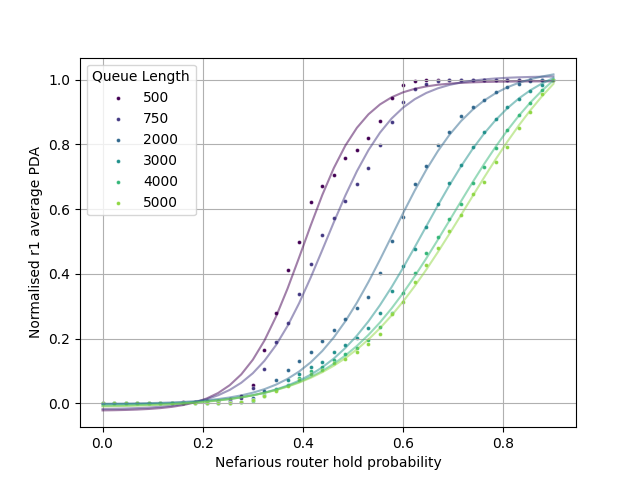
\includegraphics[width=\textwidth]{figs/results/qlen_fitting/norm_qlen_PDA_trf.png}
        \caption{Min-max scaled}
    \end{subfigure}
    \caption{Plots of average nefarious router buffer queue length over various hold probabilities fitted using TRF minimisation.}
\end{figure}

\begin{figure}[H]
    \centering
    \begin{subfigure}{0.475\textwidth}
        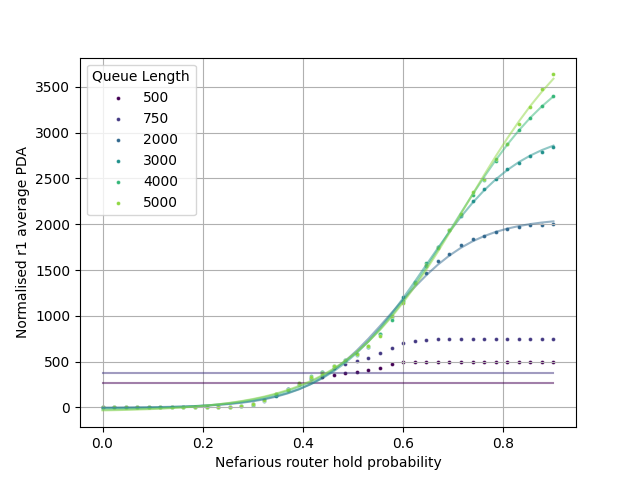
\includegraphics[width=\textwidth]{figs/results/qlen_fitting/qlen_PDA_dogbox.png}
        \caption{Original}
    \end{subfigure}
    \begin{subfigure}{0.475\textwidth}
        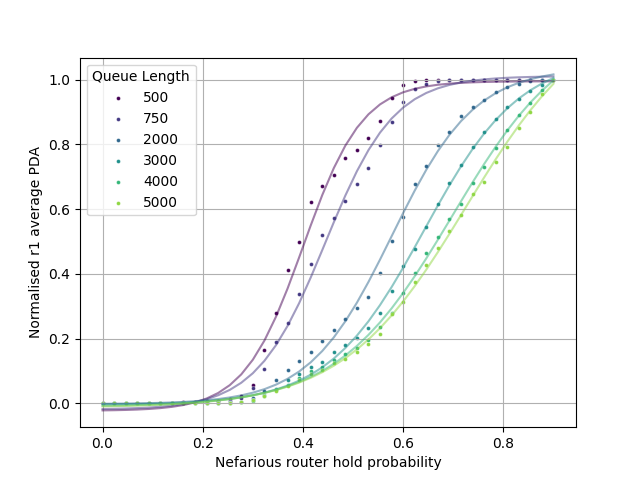
\includegraphics[width=\textwidth]{figs/results/qlen_fitting/norm_qlen_PDA_dogbox.png}
        \caption{Min-max scaled}
    \end{subfigure}
    \caption{Plots of average nefarious router buffer queue length over various hold probabilities fitted using dogbox minimisation.}
\end{figure}

\begin{table}[H]
 \centering
  \begin{tabular}{@{}cccccc@{}}
   \toprule
    &&\multicolumn{2}{c}{\textbf{PDA}} & \multicolumn{2}{c}{\textbf{PDV}} \\
    \cmidrule(rl){3-4} \cmidrule(rl){5-6}
    Algorithm & $R^2$ & Original & Scaled & Original & Scaled \\
    \midrule
    \multirow{2}{*}{LM}     & $\overline{x}$ & 99.778        & 99.778 & 99.187 & 99.187 \\
                            & min            & 99.403        & 99.403 & 98.323 & 98.323 \\
    \multirow{2}{*}{TRF}    & $\overline{x}$ & 83.211        & 99.778 & -      & 99.187 \\
                            & min            & 5.679         & 99.403 & -      & 98.323 \\
    \multirow{2}{*}{Dogbox} & $\overline{x}$ & 66.595        & 99.778 & -      & 99.187 \\
                            & min            & 6.399$e^{-9}$ & 99.403 & -      & 98.323 \\
   \bottomrule
  \end{tabular}
  \caption{Variance of nefarious router PDA grouped by varying delay probabilities in the baseline 6 router network. (Note all values are $R^2\cdot 100$)}
\end{table}